\documentclass[table]{article} % For LaTeX2e

\usepackage{hyperref}
\usepackage{url}
\usepackage{epsfig}
\usepackage{epstopdf}
\usepackage{enumerate}
\usepackage{amsmath}
\usepackage{graphicx}
\usepackage{subfigure}
\usepackage{caption}
\usepackage{tabularx}
\usepackage[table]{xcolor}
\usepackage{nips14submit_e,times}% This must be used after \usepackage[table]{xcolor} otherwise doesnt work


%\documentstyle[nips14submit_09,times,art10]{article} % For LaTeX 2.09


%\title{Fisher vector places: \\ learning compact place specific descriptors}
\title{Fisher vector places: learning compact image descriptors for place recognition}


\author{
David S.~Hippocampus\thanks{ Use footnote for providing further information
about author (webpage, alternative address)---\emph{not} for acknowledging
funding agencies.} \\
Department of Computer Science\\
Cranberry-Lemon University\\
Pittsburgh, PA 15213 \\
\texttt{hippo@cs.cranberry-lemon.edu} \\
\And
Coauthor \\
Affiliation \\
Address \\
\texttt{email} \\
\AND
Coauthor \\
Affiliation \\
Address \\
\texttt{email} \\
\And
Coauthor \\
Affiliation \\
Address \\
\texttt{email} \\
\And
Coauthor \\
Affiliation \\
Address \\
\texttt{email} \\
(if needed)\\
}

% The \author macro works with any number of authors. There are two commands
% used to separate the names and addresses of multiple authors: \And and \AND.
%
% Using \And between authors leaves it to \LaTeX{} to determine where to break
% the lines. Using \AND forces a linebreak at that point. So, if \LaTeX{}
% puts 3 of 4 authors names on the first line, and the last on the second
% line, try using \AND instead of \And before the third author name.

\newcommand{\fix}{\marginpar{FIX}}
\newcommand{\new}{\marginpar{NEW}}
\newcommand\sign[1]{\text{sign}\left(#1\right)}
\newcommand\abs[1]{\left|#1\right|}
\newcommand\norm[1]{||#1||_2}
\definecolor{myRed}{HTML}{FF3333}
\definecolor{maroon}{cmyk}{0,0.87,0.68,0.32}

%\nipsfinalcopy % Uncomment for camera-ready version

\begin{document}

%\maketitle
%***********************************************************
% *** THIS puts a figure between title and abstract ***
%\twocolumn
%[
{%
    %\renewcommand\twocolumn[1][]{#1}%
    \maketitle
    \begin{center}
        \centering
        \vspace*{-10mm}
        \fbox{\rule[-.5cm]{0cm}{4cm} \rule[-.5cm]{14cm}{0cm}}
        % \captionof{figure}
        % {
        %   Some caption 
        % }
    \end{center}%
}
%]
% ******************************************************

\begin{abstract}
%	The aim of this work is to localize a query photograph by finding other images depicting the same place in a large geotagged image database. 
%	The contributions are threefold: First, we represent each database image by a Fisher vector and for each vector we learn per-location SVM classifiers. We show that trained and re-normalized SVM weight can be used as an embedded descriptor that replaces original Fisher vector. Though the SVMs were learned independently no further calibration is necessary. We perform two experiments on state-of-the-art datasets for place recognition and we show that our method consistently improves the results for different dimensions of decorrelated Fischer vectors.
		
Exemplar support vector machines (e-SVM) are emerging as a powerful tool to learn a discriminative pre-example representation for
visual recognition. However, as individual classifiers are learnt independently for each positive example the classifier scores require careful and tedious calibration on an independent held-out data. 
The contribution of this work are three fold.
First, we analyze the e-SVM cost and show that the learnt hyperplane can be interpreted
as a new descriptor that replaces the original positive example and is re-weighted to increase its distance from the negative data.
Second, we demonstrate that after an appropriate normalization of the new re-weighted descriptor no further calibration is necessary. % of the learnt per-location E-SVMs is necessary.
Third, we apply e-SVM training to compact Fisher vector descriptors for large-scale place recognition resulting in  
a {\em discriminative} yet {\em compact} representation of each image in the database. 
Place recognition results are shown on a dataset of 25k images of Pittsburgh and demonstrate the learnt representation
consistently improves over the standard Fisher vector descriptors with different dimensions. 
\end{abstract}

\section{Introduction}

The goal of this work is to localize a query image by matching to a large database of geotagged street-level imagery.
This is an important problem with practical applications in robotics, augmented reality or navigation. 
This task is however very difficult. It is hard to distinguish different places, e.g. streets in a city, from each other. The 
imaged appearance of a place can change drastically due to factors such as  viewpoint, illumination or even changes over time.
% such as a different season, or even structural changes such as constructed or destroyed buildings. 
Finally, with the emergence of planet-scale geotagged image collections, such as Google Street-view, the image databases are becoming very large.   
We estimate a single country like France is covered by more than 60 million street-level panoramas. 
Hence the fundamental challenge in place recognition lies now in designing robust, discriminative yet compact image representations.

In this work we build on the method of Gronat {\it et al.}~\cite{Gronat13} who represent each image in the database by a per-location classifier
that is trained to discriminate each place from other places in the database. At query time, the query image is classified by all per-location classifiers and assigned to a place with the highest classification score. The training of each classifier is performed using the per-exemplar support vector machine (e-SVM)~\cite{Malisiewicz11}, which takes the positive image
as a single positive example and other far away images in the database as negative data. 
The exemplar SVM is well suited for this task as street-level image collections typically contain only one or at most hand-full of images depicting the same place. The intuition is that the exemplar SVM can learn the important features that distinguish the particular place from other similar places  in the database.  While the results of~\cite{Gronat13} are promising they suffer from two important drawbacks. First, the learnt place specific representation is not compact, 
%This is because images are represented using very high-dimensional ($d=100k$) bag-of-visual-words vectors.
 which prohibits its application to planet-scale street-level collections that are now becoming available~\cite{Klinger13}. Second, the per-exemplar classifiers require careful and time-consuming calibration.

%The exemplar support vector machine (e-SVM) has been used in a number of visual recognition tasks including
%category-level recognition~\cite{Malisiewicz11}, cross-domain retrieval~\cite{Shrivastava11}, scene parsing~\cite{Tighe13}, %image to 3D model alignment~\cite{Aubry13},
%place recognition~\cite{Gronat13} or as an initialization  for more complex discriminative clustering models~\cite{Doersch12,Singh12}. The main idea is to train a linear support vector machine (SVM) classifier from a single positive example and a large number of negatives. The intuition is that the resulting weight vector will give a higher weight to the discriminative dimensions of the positive training data point and will down weight dimensions that are non-discriminative with respect to the negative training data. A key advantage is that each per-exemplar classifier can be trained independently and hence the learning can be heavily parallelized. 
%The per-exemplar training brings however also an important drawback. As each classifier is trained independently a
%careful calibration of the resulting classifier scores on additional held out data is required~\cite{Gronat13,Malisiewicz11}. 

In this work we address both these issues. 
First, we apply the exemplar SVM training to compact Fisher vector~\cite{Jegou2011,Perronnin2010} image descriptors, which results in a {\em discriminative} yet {\em compact} representation of each image in the database.  
Second, to avoid the expensive classifier calibration we analyze the exemplar SVM cost and show that the learnt hyperplane can be interpreted
as a new descriptor that replaces the original positive example and is re-weighted to increase its distance from the negative data.
As a result of this analysis, we demonstrate that after an appropriate normalization of the new re-weighted descriptor no further calibration is necessary.

We show improved results on place recognition using learnt compact Fisher vector descriptors of different dimensionality without the need for additional calibration.  
The same procedure be potentially applied to other descriptors such as HOG~\cite{Dalal05} or the recently developed convolutional neural network features~\cite{Donahue13,Krizhevsky12,Oquab14,Sermanet13}.      

%Similar to~\cite{Gronat13}, in this work we apply exemplar SVM training to learn a location specific descriptor for large-scale place recognition in street-level image collections such as Google Street-view. This is a practically important set-up with applications in robotics, augmented reality or navigation.
%% Finding images depicting in the same place is a practially important set-up with applications    
% The exemplar SVM is well suited for this task as street-level image collections typically contain only one or at most hand-full of images depicting the same place. The intuition is that the exemplar SVM can learn the important features that distinguish the particular place from other similar places  in the database.  While the results of~\cite{Gronat13} are promising they suffer from two important drawbacks. First, the learnt place specific representation is not compact, which prohibits its application to planet-scale street-level collections that are now becoming available~\cite{Klinger13}. Second, as discussed above the per-exemplar classifiers require careful and time-consuming calibration on held-out imagery.

%In this work we address both these issues. 
%First, we apply the exemplar SVM training to compact Fisher vector~\cite{Jegou2011,Perronnin2010} image descriptors, which results in a compact yet discriminative representation of each image in the database.  
%Second, to avoid the expensive classifier calibration we analyze the exemplar SVM cost and show that the learnt hyperplane can be interpreted
%as a new descriptor that replaces the original positive example and is re-weighted to increase its distance from the negative data.
%As a result of this analysis, we demonstrate that after an appropriate normalization of the new re-weighted descriptor no further calibration is necessary.
%
%We show improved results on place recognition using learnt compact Fisher vector descriptors of different dimensionality without the need for additional calibration.  
%The same procedure be potentially applied to other descriptors such as HOG~\cite{Dalal05} or the recently developed convolutional neural network features~\cite{Donahue13,Krizhevsky12,Oquab14,Sermanet13}.      



%	Internet contains a huge collection of imagery that grows  literally every second. For instance, in 2013 Facebook claimed \cite{imageGrow} that every single minute users upload about 208,300 new images, for Instagrama this number was about  27,800. This makes about 340,000,000 new images per day. Another interesting factor is that every minute users will upload more than 100 hours of video on Youtube. Considering the fact that most of the videos are in HD make these numbers even more impressive.
%
%	Imagine that there was a system that takes a picture from the imagery as an input and it shows you a position on the map indicating where the input image was captured. What would be this system useful for? One could take a picture from his smartphone and use it as an alternative to GPS or to precise localization in urban areas when the GPS was noisy. Surely, it would find its place in security and surveillance applications where one could localize an unknown image or video sequence based on its appearance. An alternative application would be a path reconstruction from a first-person-view or UAV video \c which was cheaper then state-of-the-art SLAM. Interesting may be a localization of scenes in old movies or collecting images from one place and observe how the place has changed over time.
%
%	Indeed, many of these systems already exist \cite{Majdik2013, Torii2011} and have been intensively developed in last decade. In place recognition problems, researchers use many diverse techniques and aim for slightly different goals but the basic idea of the place recognition is the same; There is a structured collection of imagery where each image contains information about its location in the environment. This information can be for instance a GPS location or an image position in the semantic graph. Such a structured image collection is called a database. Given an unknown query image, the goal is to find the most similar image in the database and use its structural information for query localization, e.g. plot its GPS position on the map.
%
%	The structured database may contain from few thousands to couple of millions of images.  To find a similar image in the database is therefore a challenging task. As an example, the query and database images may depict the same 3D object (e.g. building) from a different camera viewpoint, under different illumination conditions or the object can be partially occluded. In addition, the database can be very large. For instance, we estimate that Google Street View of France contains more than 60 million panoramic images. Therefore, we want to represent the images by descriptors that are robust to viewpoint changes, occlusion, illumination conditions and at the same time these descriptors must be low dimensional (or very sparse) in order to perform efficient and cheap retrieval in a large database.

%%%%%%%%%%%%%%%%%%%%%%%%%%%%%%%%%
\section{Related work} 
\label{sec:related}
%%%%%%%%%%%%%%%%%%%%%%%%%%%%%%%%%

\subsection*{Large-scale visual place recognition} \vspace{-3mm}
    %- Typically using BoVW.
    %- FV has been used by Torii13, but without learning.
    The visual localization problem is typically treated as large-scale instance-level retrieval~\cite{Cummins09,Chen11,Gronat2013,Knopp2010,Schindler07,Torii2013,Zamir10}, where images are represented using local invariant
    features~\cite{Lowe04} aggregated into the bag-of-visual-words~\cite{Csurka04,Sivic03} representation. 
    The image database can be further augmented by 3D point clouds~\cite{Klinger13}, automatically
    reconstructed by large-scale structure from motion
    (SfM)~\cite{Agarwal-ICCV-2009,Klinger13}, which enables
    accurate prediction of query image camera
    position~\cite{Li12,Sattler12}.
    In this work we investigate learning a discriminative representation using the compact Fisher vector descriptors~\cite{Jegou12}.
    Fisher vector descriptors have shown excellent place recognition accuracy~\cite{Torii2013}. In this work we further
    improve their performance by discriminative learning.
    %or more recently~\cite{Torii-CVPR-2013} the Fisher vector
    %descriptor~\cite{Jegou12}.  

\vspace{-3mm}
\subsection*{Fisher vector image representations} \vspace{-3mm}
    Fisher vector image representations have recently demonstrated excellent performance for a number of visual recognition tasks~\cite{Chatfield11,Jegou12,Krapac2011,Simonyan2013}.
    They are specially suited for retrieval applications since they are robust to image appearance variations and capture richer image statistics than the simple bag-of-visual-words (BOW) aggregation. However, the raw extracted Fisher vectors are typically high-dimensional, e.g. with 32,768 non-sparse dimensions, which is impractical for large-scale visual recognition and indexing applications. Hence, their dimensionality is often reduced by principal component analysis (PCA) and further quantized for efficient indexing using e.g. product quantizer~\cite{Jegou12}.  Other recent work has demonstrated improved performance in a face recognition application by finding discriminative projection using large number of training face data~\cite{Simonyan2013}. Our work is complementary to these methods as it operates on the projected low-dimensional descriptor and further learns discriminative re-weighting of the descriptor for specific to each image in the database using per-exemplar support vector machine~\cite{Malisiewicz11}.

% In general, these results have been achieved by optimizing: 	
% 	\begin{enumerate}[(i)]
% 		\item the aggregation of local image descriptors (FV)
% 		\item the dimensionality reduction (e.g. PCA, Mahalanobis metric, whitening)
% 		\item the indexing algorithm (eg. PQ, LSH, SH)
% 	\end{enumerate}


%\paragraph{Learning discriminative projections for Fisher vectors.}
%Usually global and different tasks (faces, ...).
%We do per-exemplar training.
\vspace{-3mm}
\subsection*{Per-exemplar support vector machine} \vspace{-3mm}
    The exemplar support vector machine (e-SVM) has been used in a number of visual recognition tasks including
    category-level recognition~\cite{Malisiewicz11}, cross-domain retrieval~\cite{Shrivastava11}, scene parsing~\cite{Tighe13}, %image to 3D model alignment~\cite{Aubry13},
    place recognition~\cite{Gronat13} or as an initialization  for more complex discriminative clustering models~\cite{Doersch12,Singh12}. The main idea is to train a linear support vector machine (SVM) classifier from a single positive example and a large number of negatives. The intuition is that the resulting weight vector will give a higher weight to the discriminative dimensions of the positive training data point and will down weight dimensions that are non-discriminative with respect to the negative training data. A key advantage is that each per-exemplar classifier can be trained independently and hence the learning can be heavily parallelized. 
    The per-exemplar training brings however also an important drawback. As each classifier is trained independently a
    careful calibration of the resulting classifier scores on is required~\cite{Gronat13,Malisiewicz11}. 

%
%\paragraph{Large-scale place recognition.}
%- Typically using BoVW.
%- FV has been used by Torii13, but without learning.

\vspace{-3mm}
\subsection*{Contributions} \vspace{-3mm}
    The contributions of this work are threefold.
    First, we analyze the the exemplar support vector machine objective and show that the learnt hyperplane can be interpreted
    as a new descriptor that replaces the original positive example and is re-weighted to increase its distance from the negative data.
    Second, we demonstrate that after an appropriate normalization of the new re-weighted descriptor no further calibration is necessary. 
    Third, we apply e-SVM training to compact Fisher vector descriptors for large-scale place recognition resulting in  
    a {\em discriminative} yet {\em compact} representation of each image in the database. 
    Place recognition results are shown on a dataset of 25k images of Pittsburgh and demonstrate the learnt representation
    consistently improves over the standard Fisher vector descriptors with different dimensions. 



%
%\paragraph{Related work by P.G. }
%	Unlike the other work in large scale place recognition~\cite{Gronat2013,Cummins09,Knopp2010,Schindler07} and image retrieval~\cite{Nister06,Philbin07,Sivic2003}, we do not build on the bag-of-visual-words representation~\cite{Csurka04,Sivic2003}. Instead, we use Fisher vectors (FV) \cite{Jegou2011} that are recently finding its place in image retrieval, place recognition \cite{Torii2013} and other computer vision tasks \cite{Simonyan2013, Krapac2011}. These high-dimensional image representations are well-suited for retrieval problems since they are very robust to view-point changes and are more discriminative than standard bag-of-visual-words (BOW). However, the main drawback of FV is that unlike BOW it is dense which makes it nearly unfeasible for usage because of the memory footprint and computational cost.
%
% 	For the above-mentioned reasons researchers aim on FV optimization. As an example, a nice paper of Perronnin et al. \cite{Perronnin2010} focuses on analysis and compression of FV for image retrieval. They explain how the FV is related to BOW and underline that power-normalization of FV is equivalent to a burstiness features suppression \cite{Jegou2009}. They benefit from the fact that as the power~$\alpha$ goes to zero the {$\alpha$-normalized} Fisher vector converges to a ternary representation which can be efficiently binarized. They compared their method with the Local Sensitive Hashing (LSH) and the Spectral Hashing (SH) and showed comparable results while achieving only 520~bits signature per image. This encouraging result have been outperformed by Jegou et al. \cite{Jegou2011} who achieved comparable results with just 128~bits signature by using product quantizers (PQ). Hence, the Fisher vectors can be significantly compressed by appropriate indexing. In general, these results have been achieved by optimizing:
% 	
% 	\begin{enumerate}[(i)]
% 		\item the aggregation of local image descriptors (FV)
% 		\item the dimensionality reduction (e.g. PCA, Mahalanobis metric, whitening)
% 		\item the indexing algorithm (eg. PQ, LSH, SH)
% 	\end{enumerate}
%
% 	The lower the dimension before indexing step (iii) is the lower size of the signature is achieved after indexation. Therefore it is very important to project the FV into lower dimension. There are different methods for (ii) among which the very popular is PCA. This method, however, has a drawback. It discards uncorrelated `noisy' dimensions that can actually contain discriminative information for image retrieval.This problem have been addressed in \cite{Simonyan2013}. They use a labeled training data and utilize discriminative learning in order to learn a global low-rank metric which can be decomposed to a linear projection to low-dimensional space. Our method aim on improving the performance of the projected FV, hence it could be viewed as an intermediate step between (ii) and (iii) into the scheme above.
%
%\section{Approach overview}
%	Our setup is similar to approach of \cite{Gronat2013} where authors learn a set of per-location classifiers for place recognition, one per each location in the map. In that paper they use a BOW representation and emphasize that subsequent classifier calibration is a critical issue.  Due to the calibration procedure the method is less efficient in terms of computational cost and is hard to scale up. Need for calibration has been also reported in \cite{Malisiewicz11} where they learn per-exemplar SVM classifiers on HOG representation for object retrieval. 
%	We aim on embedding FVs in order to achieve better performance by learning. In contrast to above-mentioned papers, our method with FVs works per-se without need of any further calibration and can be therefore subsequently compressed by an indexing algorithm \cite{Jegou2011}. In addition, it does not increase the dimensionality of the problem as if it would be the case for sparse image representation.
%
% 	Rather then global approach we propose to treat FVs locally. We aim on learning a SVM weight in turn for each FV in such a way that this weight can be subsequently used as a new descriptor that replaces the original FV. Our method could be plugged into the scheme above as an intermediate step before indexing. To achieve the goal, for each FV in turn we: (i) collect hard negatives for given FV, (ii) learn a linear SVM weight (iii) and re-normalize the learned weight. At query time we compute a FV for the query image and measure its similarity with database images by computing a dot-product between the FV and each of the re-normalized SVM weights. We observe that learned re-normalized weight does not differ to much from the original FV. Loosely speaking, we embedded the information about hard negative exemplars into the original FV. The details will be given later in the text.
%
% 	
%	The main contributions of this paper are as follows: 
%	We show that trained and re-normalized SVM weight can be used as an embedded descriptor that outperforms the original one without need for further calibration. We perform two experiments on state-of-the-art dataset for place recognition and we show that our method consistently improves the results for (i) different PCA dimensions and (ii) over all recall@K metric shortlist, i.e. the rate of relevant images that are ranked in top K positions.
%
%	The rest of the paper is organized as follows:
%	In section \ref{sec:FV} we first give a brief overview of FV implementation for image retrieval. Then, in section \ref{sec:perExemplar}, we the explain how the per-location classifiers are trained  and finally in section \ref{sec:exp} we present our experimental results along with implementation details.
%
%

%%%%%%%%%%%%%%%%%%%
\section{Fisher vector overview}
\label{sec:FV}
%%%%%%%%%%%%%%%%%%%
	The Fisher vector can be thought of as an extension of BOW \cite{Sivic2003} that is achieved by considering a high-order statistics of the distribution of the feature descriptors. It aggregates a large set of descriptors into a high-dimensional representation of the fixed size. In the following text we briefly overview some basic concepts of Fisher vectors, its normalization and standard dimensionality reduction.

	\subsection{Computing Fisher vectors}
		It first starts with learning a generative model of the local image descriptors $x$ of the dimension~$d$ (in our case we use SIFT features, see details in Sec. \ref{sec:exp}). The model is assumed to follow a GMM with $N$ components and diagonal covariances. This model can be understood as a probabilistic visual vocabulary. Having the model trained, the Fisher vector of the sample of the image descriptors is computed as a gradient of the sample's likelihood with respect to the learned parameters of the GMM, which is subsequently scaled by inverse square root of the Fisher information matrix \cite{Perronnin2007}. Considering only the derivatives w.r.t. the mean and covariances, we a obtain representation which captures the average of the first and second order differences between the descriptors and each of the GMM center $k$. For the image containing $T$ feature vectors it can be expressed as follows:
		
		\begin{align}
			\Phi^{(1)}_k&=
			\dfrac{1}{N \sqrt(w_k)}\sum_{j=1}^{T} \alpha_j(k) \left(
			\dfrac{x_j-\mu_k}{\sigma_k}
			\right)
			\label{eq:FVmean}
			\\
			\Phi^{(2)}_k&=
			\dfrac{1}{N \sqrt(2w_k)}\sum_{j=1}^{T} \alpha_j(k) \left(
			\dfrac{(x_j-\mu_k)^2}{\sigma_k^2}-1 
			\right)
			\label{eq:FVvar}
		\end{align}

		\noindent
		where $w_k, \mu_k$ and $\sigma_k$ are weight, mean and diagonal of covariance matrix for $k$-th component of the learned GMM and $\alpha_j(k)$ is a soft assignment of the $j$-th feature $x_j$ to the Gaussian $k$. The resulting Fisher vector  $\Phi$ is then concatenation of these gradients which forms into a $2Nd$ dimensional vector such that $\Phi=[\Phi^{(1)T}_1,\Phi^{(2)T}_1,...,\Phi^{(1)T}_N,\Phi^{(2)T}_N]^T$.

		While some works, e.g.\cite{Perronnin2010}, use only a partial derivatives w.r.t. the mean parameters (equation~\eqref{eq:FVmean}), we use partial derivatives both w.r.t. the mean and variance because this approach have been implemented in a library that we used (details are provided in section \ref{sec:exp}). As reported in \cite{Jegou2010} both approaches provide comparable results.

		\subsection{Normalization}
			As in the case of standard BOW, Fisher vector is typically $L2$ normalized in order to measure similarity between two FVs by a dot-product. However it has been shown that direct $L2$ normalization is suboptimal and better performance can be achieved by power-normalization followed by $L2$ normalization. Thus the normalization operator can be written as follows:
			
			\begin{equation}
				L(z)=\dfrac{\text{sign} (z) \abs{z}^\alpha}{\norm{\text{sign}(z) \abs{z}^\alpha}}
				\label{eq:Loperator}
			\end{equation}

			\noindent
			where $\alpha \in (0,1)$ is an element-wise power and $z \in R^d$ is an arbitrary real vector. As mentioned in the introduction, the power-normalization has the effect of suppression of the descriptors that occur frequently in the image (bursty features), these can be for instance periodical structures such as skyscraper windows or bricks of the wall. In our setup we use $\alpha=0.5$ as it has been reported by Jegou et al. \cite{Jegou2012HAL} that this value is optimal for wide range of GMM components $N$.

		\subsection{Dimension reduction}
			The resulted Fisher vector is a high-dimensional representation of an image, which dimensionality depends only on number of $N$ components of the GMM and dimension $d$ of the local image descriptors which is fixed. In practice, the PCA is being used for decorrelation and projection to a lower dimensional space because it subsequently directly affects a size of the indexed signature (see Sec. \ref{sec:overview} and \cite{Jegou2011}).

			We observed that after the PCA decorrelation it is important to $L2$ re-normalize projected FV to achieve better performance. Our interpretation is that after performing the PCA the higher dimensions contain a noise that affects only a magnitude of the projected vectors but not its direction. Furthermore we observed that even slightly better results can be achieved by using the normalization operator \eqref{eq:Loperator} instead of $L2$.

			Finally, it is worth noting that PCA projection into a `not-too-low' dimensional space can actually slightly improve the performance of the full FV. What that `not-too-low' actually means have been partially discussed in \cite{Jegou2012HAL}. However, in general as the dimension decreases the performance of decorrelated FV decrease which is, indeed, what we observe in our experiments. In the next section we therefore aim on enhancing the performance of projected FVs.   


%\section{Per-exemplar SVM and Fischer vectors}
%%%%%%%%%%%%%%%%%%%%%%%%%%%%%%%%%%%%%%
\section{Learning compact place descriptors using per-exemplar SVM}
%%%%%%%%%%%%%%%%%%%%%%%%%%%%%%%%%%%%%%
\label{sec:perExemplar}
	Each database image $j$ is represented by its L2-normalized Fisher vector $\Phi_j$. The goal is to learn a set of new L2-normalized Fisher vectors $\Psi_j$, one per each database image, such that at query time, given the Fisher vector $\Phi_q$ of an unknown query image, we retrieve the database image depicting the same location by finding the image $j^*$ with the highest score measured by a dot product
	\begin{equation}
	    j^*=\operatorname*{arg\;max}_{j} \Phi_q^T \Psi_j. 
	    \label{eq:class}
	\end{equation}
%	Note that both the query and database vectors are L2 normalized and hence the dot product measures the cosine of   
	In other words, the aim is to replace each original database Fisher vector $\Phi_j$ with a new vector $\Psi_j$ that is more discriminative in the sense of separation from descriptors of images depicting other places. 
	Inspired by~\cite{Gronat2013} we investigate applying the exemplar support vector machine (e-SVM)~\cite{} for this task. 
	e-SVM learns a linear classifier $w_j^T\Phi+b_j$ given the descriptor of place $j$ as a single positive example $\Phi_j^+$ and a large number of negative data $\mathcal N_j$ from other places in the database.
	The intuition is that the resulting weight $w_j$ vector will give a higher weight to the dimensions of the descriptor that are discriminative and will down-weight dimensions that are non-discriminative with respect to the negative training data collected from other far-away places.  The optimal $w_j$ and $b_j$ are obtained
	by minimizing the following convex objective  
%	The vector should have a unit $L2$-norm in order to measure the distance by a dot-product in equation \eqref{eq:class}. 
%	In the following we analyze a limit behavior of per-exemplar SVM convex objective and show that learned hyperplane normal can be interpreted as a new descriptor that increases the measured distance from negative data.
        \begin{equation}
	        ||w_j||^{2} +C_1 \cdot h
	        				\left(
	        				w_j^T\Phi^+_j+b_j
	        				\right)
	                         +C_2\sum_{\Phi\in \mathcal N_j}h
	                         \left(
	                         -w_j^T\Phi-b_j
	                         \right), 	
	       	\label{eq:obj} 
	  	\end{equation}

	  	where $\Phi^+_j$ is the descriptor of the place $j$ as a the positive data point, $\Phi$ are Fisher descriptors from negative training data $\mathcal N_j$ and $h$ is the hinge loss. Note that the first term $||w_j||$ is the regularizer, the second term is the loss on the positive data weighted by scalar parameter $C_1$ and the third term is the loss on the negative data weighted by scalar parameter $C_2$. The optimal parameters $w_j$ and $b_j$ can be obtained using standard software packages such as~\cite{libsvm}. A key advantage is that the per-exemplar classifier for each place can be trained independently and hence the learning can be heavily parallelized. On the downside, as the individual per-location classifiers are trained independently the resulting scores have to be calibrated with respect to each other on additional data~\cite{Gronat13,Malisiewicz11}.

        In the following section, we analyze the exemplar SVM objective~(\ref{eq:obj}) and show the learnt \textcolor{myRed}{and re-normalized} weight vector $w_j$ can be interpreted as 
        a new descriptor $\Psi_j$.  In particular, when the weight $C_2$ of the negative data in objective~(\ref{eq:obj}) goes to zero the $\Psi_j$ is going to be identical to original $\Phi_j^+$.  As $C_2$ increases $\Psi_j$ goes away from $\Phi_j^+$ such that the measured distance between $\Psi_j$ and negative examples increases.
        Details are given next.

% for c2->0, w_j is parallel with Phi+
% for c2>0 the direction of  w_j changes such as the dot-product is maximied
% this permits an intuitive intepretation of w as a new descriptor.
   		
		
%The per-exemplar training brings however also an important drawback. As each classifier is trained independently a
%careful calibration of the resulting classifier scores on additional held out data is required~\cite{Gronat13,Malisiewicz11}. 

		
%%		 $h$ is the hinge loss, and $C_1$, $C_2$ are weights for the loss on the positive or negative data. This objective is being minimized in $w_j$ and $b_j$. 
%		 In the section below will show that the new descriptor $\Psi_j$ can be interpreted as unit normal of the learned hyperplane $w_j$ and we will show that when $C_2$ in equation~(\ref{eq:obj}) goes to zero the new descriptor $\Psi_j$ is going to be identical to original $\Phi_j^+$, as $C_2$ increases $\Psi_j$ declines from $\Phi_j^+$ such that the measured distance between $\Psi_j$ and negative examples increases.
	
%	\subsection*{Per-exemplar SVM learning}\vspace{-0.2cm}
%        Per-exemplar SVM relies on a large number of negative data and only single or very few positive examples. This setup is well suited for place recognition since tipically only one positive training data is available. We follow the approach of \cite{Gronat2013} and we use per-exemplar SVM to learn a new descriptor $\Psi_j$ independently for each image in turn. The objective of per-exemplar SVM that can be written as 
%		\begin{equation}
%	        ||w_j||^{2} +C_1 \cdot h
%	        				\left(
%	        				w_j^T\Phi^+_j+b_j
%	        				\right)
%	                         +C_2\sum_{\Phi\in \mathcal N_j}h
%	                         \left(
%	                         -w_j^T\Phi-b_j
%	                         \right) 	
%	       	\label{eq:obj} 
%	  	\end{equation}
%	  	where $\Phi^+_j$ is a single positive exemplar, $\Phi$ are FVs from negative training data $\mathcal N_j$, $||w_j||$ is a regularization term, $h$ is a penalty function and $C_1$, $C_2$ are penalty weights for positive or negative data. This objective is being minimized in $w_j$ and $b_j$. In the section below will show that the new descriptor $\Psi_j$ can be interpreted as unit normal of the learned hyperplane $w_j$ and we will show that when $C_2$ in equation~(\ref{eq:obj}) goes to zero the new descriptor $\Psi_j$ is going to be identical to original $\Phi_j^+$, as $C_2$ increases $\Psi_j$ declines from $\Phi_j^+$ such that the measured distance between $\Psi_j$ and negative examples increases.
%	
	
	\subsection*{Analysis of per-exemplar SVM objective} \vspace{-0.2cm} 

        The goal is to show that the limit case behavior of the e-SVM objective \eqref{eq:obj} is such that as $C_2$ goes to zero the resulting hyperplane vector $w_j$ is parallel with the training descriptor $\Phi_j^+$. Moreover, if $w_j$ is normalized these vectors are identical.

		First, let us decompose $w_j$ into parallel and orthogonal part w.r.t. $\Phi^+$. Second, let $C_2\rightarrow 0$ and analyze the behavior of the objective. After the decomposition of $w_j$ such that $w_j=w_j^{\perp}+w_j^{||}$ the convex objective can be re-written as follows

	  	\begin{equation}
	  		\nonumber
	        ||w_j^{\perp}+w_j^{||}||^{2} +
	        C_1 \cdot h
	        \left(
	        	(w_j^{\perp}+w_j^{||})^T\Phi^+_j+b_j
	        \right)+
	        C_2\sum_{\Phi\in \mathcal N_j} h
	        \left(
	        	-(w_j^{\perp}+w_j^{||})^T\Phi-b_j
	        \right)
            \label{eq:decomposedOrig}
	   \end{equation}

	  	Notice that in the second term the orthogonal part does not change the value of a dot-product since $(w_j^{\perp}+w_j^{||})\Phi^+=w_j^{||}\Phi^+$, hence the equation \eqref{eq:decomposedOrig} becomes

        \begin{equation} 
            ||w_j^{\perp}+w_j^{||}||^{2} +
            C_1 \cdot h
            \left(
                w_j^{||T}\Phi^+_j+b_j
            \right)+
            C_2\sum_{\Phi\in \mathcal N_j} h
            \left(
                -(w_j^{\perp}+w_j^{||})^T\Phi-b_j
            \right) 
            \label{eq:decomposed} 
        \end{equation}  

         Because $C_2 \rightarrow 0$ the first two terms dominate the equation \eqref{eq:decomposed} thus in the limit case it follows that

		  	\begin{align}
      %           \nonumber
		  		% ||w_j||^2 +C_1 \cdot 
		    %     h
		    %     \left(
		    %     	w_j^T\Phi^+_j+b_j
		    %     \right)&=\\
		        ||w_j^{\perp}+w_j^{||}||^{2} +
		        C_1 \cdot h
		        \left(
		        	w_j^{||T}\Phi^+_j+b_j
		        \right)
		        &\geq
		        ||w_j^{||}||^2 +C_1 \cdot 
		        h
		        \left(
		        	w_j^{||T}\Phi^+_j+b_j
		        \right)
		       	\label{eq:bound} 
		  	\end{align}

		The inequality \eqref{eq:bound} can be interpreted such that in the limit case, for arbitrary vector $w_j$, it's parallel part always minimizes the objective. Hence, the in the limit case the $w_j$ converges to be parallel with $\Phi^+$. Also notice, that for $C_2=0$ the solution is unique such that $||w_j||=0$ and $b_j=-1$. The effect of decreasing the parameter $C_2$ is illustrated in figure \ref{fig:C2effect}.

\begin{figure}[t]
    \begin{center}
        \subfigure[]{
            \centering
            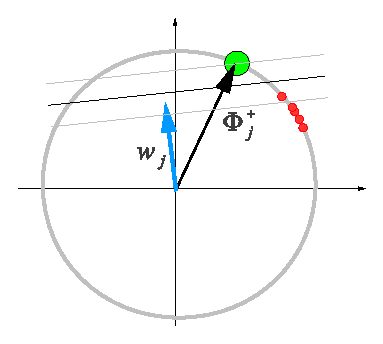
\includegraphics[width=0.35\linewidth]{imgs/figSVM01tight}
        }
        $C_2 \rightarrow 0$
        \subfigure[]{
            \centering
            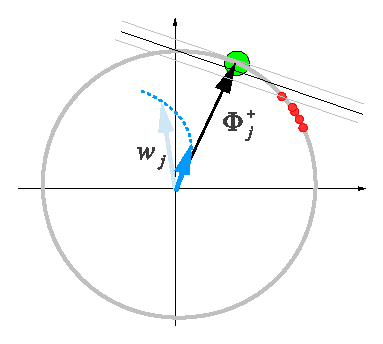
\includegraphics[width=0.35\linewidth]{imgs/figSVM02tight}
        }
    \caption{An illustration of the effect of decreasing a parameter $C_2$. As the paramterer $C_2$ decreases the resulting vector $w_j$ is being parallel to $\Phi_j^+$. Re-normalized $w_j$ is then identical with original positive vector.}
    \label{fig:C2effect}
    \end{center}
\end{figure}

	\subsection*{Interpretation, re-normalization} \vspace{-0.2cm}
	  	The result above shows that as $C_2$ decreases the normal of the hyperplane that separates the positive exemplar from negative data tends to be parallel with $\Phi^+$ as shown in figure \ref{fig:C2effect}. As $C_2$ grows, this normal declines such that distance from the negative data increases.

		Since FVs are $L2$ normalized our goal is to measure the similarity between two descriptors by an angle, equation \eqref{eq:class}, hence we interpret the new descriptor $\Psi_j$ as a normalized hyperplane normal such that

		  	\begin{equation}
		  		\Psi_j=\dfrac{w_j}{||w_j||}
		  	\end{equation}

        Notice that as $C_2$ goes to zero, the vector $\Psi_j$ becomes to be original Fisher vector $\Phi_j^+$. When $C_2$ increases the penalty term for negative data declines the vector in such way that negative training data are better separated. Loosely speaking, $C_2$ designates amount of information about discriminative and informative dimensions in the new descriptor $\Psi_j$.



    \subsection{Training data}
      	The negative training data set contains hard negative examples of the image $j$. These hard negatives are database images that are spatially far-away from image $j$ and, at the same time, have a high similarity score with image $j$ measured by a dot-product of its FVs. This approach follows the simple idea of \cite{Knopp2010} that far-away images do not share the same visual content. A GPS information associated with each database image allows us to construct such a negative set for each image $j$ in turn. Details are provided in experimental section \ref{sec:exp}.

      	The positive training data set is represented by the only image $j$ itself. Why is that? It comes from the nature of the dataset. One could find additional positive examples by taking adjacent panorama images and building a graph where each node represents an image and each edge represents a visual overlap. However, due to the panorama sampling density during the capturing process of the Google Street View it is very rare to detect a visual overlap between two adjacent panoramas. Instead, very often the detected visual overlap is between the images that come from the same panorama and differ by a homography. We found that there is no benefit from taking these images into account.

% \section{Why does exemplar-SVM works}
%   	The convex objective \eqref{eq:obj} consist of regularization term a two penalty terms with weights $C_1$ and $C_2$. We will show that if $C_2 \rightarrow 0$ the resulting $w_j$ is going to be parallel with $\Phi_j^+$, hence $\Psi_j \rightarrow \Phi^+_j$.

%   	Lets assume for the moment that the weight of the negative data penalty $C_2 \rightarrow 0$. Then the regularization term and the first penalty term dominates the equation \eqref{eq:obj}. Any arbitrary vector $w_j$ can be decomposed into parallel and orthogonal direction w.r.t. $\Phi_j^+$ such that $w_j=w_j^{\perp}+w_j^{||}$, hecnce the convex objective \eqref{eq:obj} can be rewritten as

%  	\begin{align}
%         ||w_j^{\perp}+w_j^{||}||^{2}& +C_1 \cdot h((w_j^{\perp}+w_j^{||})^T\Phi^+_j+b_j)
%                          +C_2\sum_{\Phi\in \mathcal N_j}h(-(w_j^{\perp}+w_j^{||})^T\Phi-b_j) 	
%        	\label{eq:decomposed} 
%   	\end{align}

%   	If the orthogonal part $w_j^{\perp}$ was removed the equation \eqref{eq:decomposed} becomes

%  	\begin{align}
%         ||w_j^{||}||^{2}& +C_1 \cdot h(w_j^{||T}\Phi^+_j+b_j)
%                          +C_2\sum_{\Phi\in \mathcal N_j} h(-w_j^{||T}\Phi-b_j) 	
%        	\label{eq:removed} 
%   	\end{align}

%   	Notice that this operation has affected only two terms. The negative data penalty term has changed, however this change was negligible since $C_2 \rightarrow 0$. The regularization term always decreases, while the positive data penalty term does not change due to the orthogonality. This means that as we decrease the penalty weight $C_2$ the optimal $w_j^*$ is close to being parallel with the original Fisher vector $\Phi_j^+$ as shown in Figure \ref{fig:C2effect}. The re-normalized $w_j^*$ is therefore almost identical with $\Phi^+$. As we increase the weight $C_2$ the optimal $w_j^*$ declines from the original FV and this declination depends on (i) distribution of the negative data and (ii) the value of $C_2$ w.r.t. $C_1$ Loosely speaking, the parameter $C_2$ designates how much information about hard negative examples wil be embedded in $w_j^*$.



%   	As a conclusion, for certain setting of the parameters $C_1$ and $C_2$ the learned $w_j^*$ is slightly declined from the original Fisher vector in such a way that it is better separated from the hard negative examples. The details of picking the parameters are given in the following section.

%   	\textcolor{myRed}{(TODO: In Results show (i) how much it differs e.g. dot product with original FV, (ii) how the performance changes with C2 e.g. x-validation plot or just plot.)}

\section{Experimental evaluation}
\label{sec:exp}
	In this section we first describe the experimental datasets, then we give implementation details and finally compare performance of the proposed approach on two datasets with several baseline methods.

	%%%%%%%%%%%%%%%%%%%%%%%%%%
   	\subsection{Image datasets}
   	%%%%%%%%%%%%%%%%%%%%%%%%%%
		We performed our experiments on a database of Google Street View images from the Internet. For evaluation we have used two datasets. The first one is identical to \cite{Gronat2013, Torii2011} ($25k$ of images), the latter one is an extension extension of this dataset to achieve a higher spatial density ($55k$ of images).

		We downloaded panoramas from Pittsburgh (U.S.) covering roughly an area of $1.3 \times 1.2 \; {\rm km}^2$. Similar to~\cite{Chen11}, for each panorama we generate 12 overlapping perspective views corresponding to two different elevation angles to capture both the street-level scene and the building fa\c{c}ades, resulting in a total of 24 perspective views each with $90^\circ$ FOV and resolution of $960 \times 720$ pixels.

		As a query set with known ground truth GPS positions, we use the 8999 panoramas from the Google Street View research dataset, which cover approximately the same area, but were captured at a different time, and typically depict the same places from different viewpoints and under different illumination conditions. For each test panorama, we generate perspective images as described above. Finally, we randomly select out of all generated perspective views a subset of 4k images, which is used as a test set to evaluate the performance of the proposed approach.



\begin{figure}[t!]
    \centering
    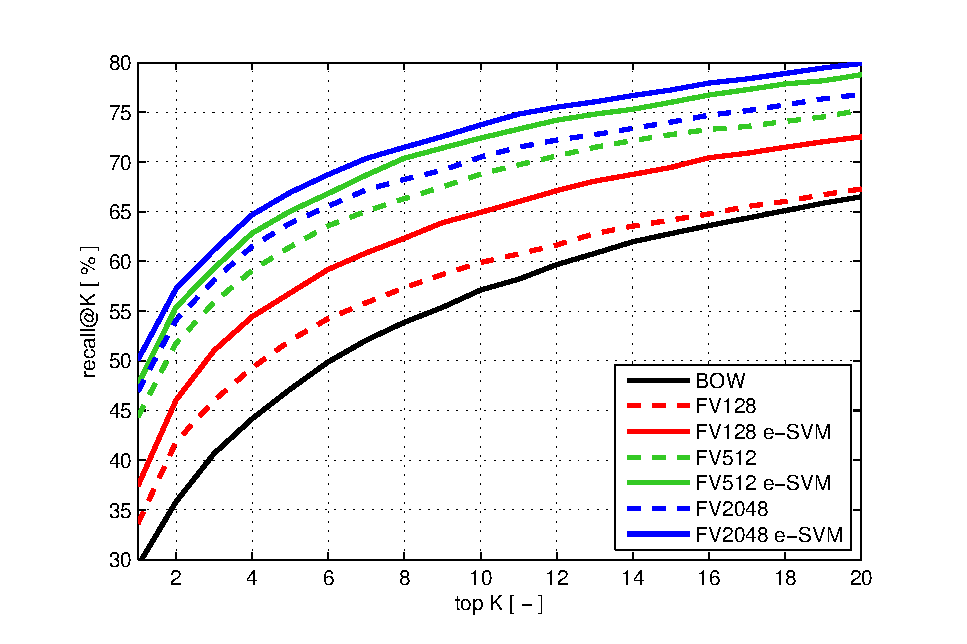
\includegraphics[width=\linewidth]{imgs/plotPitt25k}    
    \caption{
        \textbf{Evaluation on Pittsburgh 25k \cite{Gronat13} dataset.} The fraction of correctly recognized queries (recall@K, y-axis) vs. the number of topK retrieved datbase images for different FV dimensions. Proposed method (e-SVM) consistently improves the results over all dimensions.
    }
    \label{fig:recall}
\end{figure}

	%%%%%%%%%%%%%%%%%%%%%%%%%%%%%%%%%%%
   \subsection{Implementation details}
   %%%%%%%%%%%%%%%%%%%%%%%%%%%%%%%%%%%
	   	\paragraph{SIFT features:}
	   		For all images in turn SIFT local descriptors~\cite{Lowe04} are extracted and subsequently these features are converted to a rootSIFT \cite{Arandjelovic12}. For extraction we use publicly available library {\tt vlfeat}~\cite{vlfeat}.
	    
	    \vspace{-4mm}
	   	\paragraph{BOW baseline:}	
	    	A vocabulary of 100k visual words is learned by approximate k-means clustering~\cite{Philbin07} from a subset of features from 5,000 randomly selected images. A tf-idf~\cite{Sivic2003} vector is computed for each image by assigning each descriptor to the nearest cluster center.  Finally, all tf-idf vectors are normalized to have unit $L_2$ norm.

	    \vspace{-4mm}
	    \paragraph{Fisher vector baseline:}
	    	We first begin with decorrelation of local descriptors. We train a PCA matrix on a set of descriptors of 5,000 randomly selected database images and we project all rootSIFT descriptors into a $d=64$ dimensional space. Then we learn a generative GMM that consist of $N=256$ components. We train this model on a set of decorrelated descriptors from 5,000 randomly selected database images.

	    	It follows by learning a PCA for FV decorrelation. The resulting dimension of full FV is $2Nd=32,768$. To learn a reasonable non-singular PCA matrix we need at least this amount of data which we do not have for the first dataset which consists of only 25k images. For both databases we use all available data to train the PCA and we underline that for the first $25k$ dataset the projection to $d'>25k$ is meaningless since the PCA matrix was singular.

	    	Finally, to compute the FV of an image we (i) compute the rootSIFTs and perform the PCA decorrelation to $d=64$ space, (ii) use the learned GMM and decorrelated descriptors to compute full FV (iii) project the full FV into lower dimensional spaces, namely to $2^\beta$ where $\beta=7\dots 14$ and (iv) re-normalize projected FVs by operator \eqref{eq:Loperator}.

	    \vspace{-4mm}
	    \paragraph{Learning vectors:}
			To learn the linear regressor \eqref{eq:linreg} for database image $j$, the positive and negative training data is constructed as follows. 
			The \emph{negative training set} $\mathcal N_j$ is obtained by: (i) finding the set of images with geographical distance greater than $200{\rm m}$; (ii)  sorting the images by decreasing value of similarity to image $j$ measured by the dot product between their respective Fisher vectors; (iii) taking the top $N=500$ ranked images as the negative set. 
			In other words, the negative training data consists of the hard negative images, i.e. those that are very similar to image $j$ but are far away from its geographical position, hence, cannot have the same visual content. The \emph{positive training set} $\mathcal P_j$ consist of the only image $j$ itself.

			For SVM training we use {\tt libsvm} \cite{libsvm} with $L2$ regularizer and $L2$-loss penaty fucntion $h(x)$ from equation \eqref{eq:obj}. To obtain parameters $C_1$ and $C_2$ we perform a grid search and evaluate the performance on held out test set. We observe that for different FV target PCA dimensions the parameter $C_1$ is quite stable (typically $C_1=1$) while the optimal parameter for $C_2$ differs between $10^{-6}$ to $10^{-1}$.

			To learn the new image representation from FVs, for each database image $j$ in turn we (i) learn SVM from $\mathcal P_j$ and $N_j$ (ii) $L2$ normalize learned $w_j$ (iii) use this vector as the new image representation. At query time we compute a FV $\Phi_q$ of the query image and measure its similarity score to each database image by equation \eqref{eq:linreg}.
		
		\vspace{-4mm}
		\paragraph{Ground truth:}
			Since all the query images have associated GPS location we can compute the spatial distance from database image. We consider query image to be correctly localized if its retrieved database image lies within a perimeter of $20m$ from the query image.


	\subsection{Results}
		For each database we compare our results to two baselines: a standard BOW baseline and a Fisher vector baseline. We measure our performance by recall@K metric which is the portion of query images that have at least one relevant image inside its ranked shortlist of the length $K$. We perform our experiments on several target FV dimensions as shown in the figure \ref{fig:recall}.

		It is noticeable that proposed method outperforms all baselines and consistently improves the performance of the original FV over all lengths $K$ of the shortlist and all target FV dimensions. This particularly means that learned descriptors are more likely to attract relevant images into top$K$ shortlist. The results are summarized in table \ref{tab:recall}.

\begin{table}[t!]
\begin{centering}
	\begin{tabularx}{0.94\linewidth}{|c|c c c c c|c c c c c|}
		\hline 
		\rowcolor{maroon!50}
		Method: & \multicolumn{5}{c|}{25k Pittsburgh} & \multicolumn{5}{c|}{55k Pittsburgh} \\
		\hline 
		\hline 
		\rowcolor{maroon!50}
		recall@K [$\%$] & 1 & 2 & 5 & 10 & 20 & 1 & 2 & 5 & 10 & 20\\
		\hline
		\rowcolor{maroon!10}
		BOW & 29.4 & 35.7 & 47.0 & 57.1 & 66.5 &  &  &  &  & \\
        \hline
		\rowcolor{maroon!10}
		FV128         & 33.6 & 41.8 & 52.0 & 59.8 & 67.7 & 10.9 & 14.1 & 20.2 & 26.4 & 33.2 \\
		\rowcolor{maroon!10}
		\textbf{FV128 e-SVM}   & \textbf{37.8}  & \textbf{46.1} & \textbf{56.9} & \textbf{64.9} & \textbf{72.6}  &
                                 \textbf{13.5}  &  \textbf{17.7}  &  \textbf{25.0}  &  \textbf{31.8}  &  \textbf{39.0} \\
        \hline
        \rowcolor{maroon!10}
        FV512         & 44.3 & 51.7 & 61.4 & 68.7 & 75.2 & 17.3 &  21.1 &  28.4 &  34.2 &  40.3 \\
        \rowcolor{maroon!10}
        \textbf{FV512 e-SVM}   & \textbf{47.6}  & \textbf{55.4} & \textbf{65.1} & \textbf{72.4} & \textbf{78.8}  &
                                 \textbf{19.8} &  \textbf{25.1} &  \textbf{32.7}  & \textbf{38.7} &  \textbf{46.0} \\
        \hline
		\rowcolor{maroon!10}
		FV2048        & 46.9  & 54.1 & 63.8 & 70.5 & 76.8 & 19.2 & 23.5 & 29.9 &  35.2 &  41.9 \\
		\rowcolor{maroon!10}
		\textbf{FV2048 e-SVM}  & \textbf{50.2} & \textbf{57.3} & \textbf{67.0} & \textbf{73.8} & \textbf{78.0} &
        \textbf{20.8} & \textbf{25.9} & \textbf{33.1} & \textbf{38.7} & \textbf{45.9}\\
        \hline
  %       \rowcolor{maroon!10}
  %       FV8192        & 46.0  & 52.7 & 62.5 & 69.4 & 76.4 & - & - & - & - &  -   \\
  %       \rowcolor{maroon!10}
  %       \textbf{FV8192 e-SVM}  & \textbf{48.4} & \textbf{55.6} & \textbf{65.4} & \textbf{72.6} & \textbf{79.0} & - & - & - & - & -\\
		% \hline
	\end{tabularx}
	\caption{ \textcolor{myRed}{}
		The percentage of correctly localized test queries for which the topK ranked database image is within $20$ meters from the ground truth query position. The proposed method (svmFV) outperforms the baseline methods.
		}
	\label{tab:recall}
\end{centering}
\end{table}


\section{Conclusions}





\small{
	\bibliographystyle{spmpsci}
	\bibliography{shortstrings,vggroup,cvww_template,mybib}
	}


\end{document}
